\chapter{Il benchmark}
Il problema della saturazione verrà affrontato su un sistema meccanico reale. Il sistema nasce a scopi didattici per provare architetture di controllo su un sistema lineare. Una foto dell'apparato sperimentale è mostrata in Figura \ref{fig:fotosetup}.
\begin{figure}
	\centering
	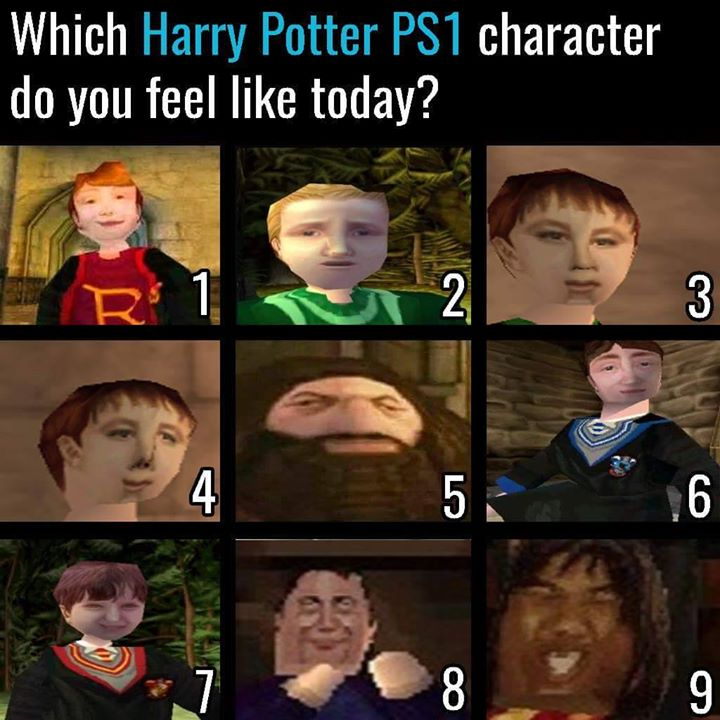
\includegraphics[height=0.5\linewidth]{img/foto_setup}
	\caption{Foto dell'apparato sperimentale (\treM)}
	\label{fig:fotosetup}
\end{figure}
\section{descrizione dell'apparato sperimentale}
Il \treM si compone di tre carrelli posizionati su tre binari. I binari sono allineati e perciò i carrelli sono vincolati a muoversi solo lungo questo asse. Ogni carrello prevedere la possibilità di essere caricato cn un numero da $0$ a $4$ masse da circa $500 \ g$.
%TODO vedi se aggiungere foto di carrello singolo e pinion rack



